\documentclass{mm2}
\usepackage{bbm}
\usepackage{bbold}
\usepackage{amsmath}
\usepackage{dsfont}
\usepackage{pdfpages}
\usepackage{amssymb}

\usepackage{amsthm,thmtools,xcolor}
\numberwithin{equation}{section}

\theoremstyle{definition}
\newtheorem{definition}{Definition}[section]

% FILL THIS WITH YOUR CIS USERNAME
\cisid{lhtp39} 
\title{Zombies}
 
\begin{document}
	\newpage
	\tableofcontents
	\newpage
\section{Introduction}
\subsection{Equilibrium}
Instead of looking at how a population changes over time, we might just wamt to look at how the popluation will end up given suffiecient time. \newline
\begin{definition}{\textbf{(Equilibrium)}} The equilibrium of a system is where all time derivitives vanish. For example consider the system
	\begin{eqnarray}
	\frac{d^2x}{dt^2} = 2x^2 + 2y^2, \hspace{1cm} \frac{d^2y}{dt^2} = 2xy.
	\end{eqnarray} 
	Then the equations of equibria are 
	\begin{eqnarray}
	2x^2 + 2y^2= 0, \hspace{1cm} 2xy= 0.
	\end{eqnarray}
	The solution to these equations is when $x=y=0$.
\end{definition}
\begin{definition}{\textbf{(Permissible equilibrium)}} As we are looking at populatiosn and you can't have a negative popultaion we say that the population is $\geq 0$, we define a permissible equilibrium as one which solves this criteria.
\end{definition}
\begin{definition}{\textbf{(Stability)}} We say an equilibrium is stable if it returs to its original position after being disturbed. For example any small change from $x=y$ (eg $x = y + \epsilon$) will tend back to $x=y$ exponentially fast.
\end{definition}
\begin{definition}{\textbf{(Unstability)}} We say an equilibrium is unstable if it doesnt return to its original position after being disturbed. For example a small change from $x=y$ (eg $x = y + \epsilon$) won't tend back to $x=y$.
\end{definition}
\subsection{The pendulum equation and stability}
To see if a system is stable or not, we can perform linear stability analysis, by looking at the neighbourhood of the fixed point equiibria. Before we give a breakdown at this technique we willlook ath epedulum equation.
\subsubsection{Pendulum equation}
Tobegin with we consider a rigid pendulum as shown in FIGURE, which has a bead of mass m attatched to a rigid rod of length l. The force from gravity g given the rod makes an angle $\theta$ to the vertical has two components $-mg\sin\theta$ along the direction of swing $\frac{d\theta}{dt}$ and the component along the axis of the rod which is balanced by the rods tension $T$ balances the weight along its length. there is also a frictional force which we model as $\nu\frac{d\theta}{dt}$, with $\nu$ the coeffiencient of friction between the pendulum bead and the surrounding medium (air). The velocity is the change in arclength $l\theta$, $l\frac{d\theta}{dt}$ and hence the acceleration $a = l \frac{d^2 \theta}{dt^2}$. Using Newton's law we have
\begin{eqnarray}
F = ma \implies \frac{d^2 \theta}{dt^2} + \frac{\nu}{m}\frac{d\theta}{dt} + \frac{g}{l}\sin\theta =0.
\end{eqnarray}
Our physical intuition tells us that the pendulum will swing with a decreasing amplitude untill it relaxes to $\theta = 0$. As shown in FIGURE. There are two equibria to this system , taking into accunt periodicity, $\theta(t) = 0 \forall t$ and $\theta(t) = \pi \forall t$. The solution $\theta = 0$ corresponds to the pendulum starting at the bottom of its cycle and not moving. The solution $\theta = \pi$ corresponds to when the pendulum rod is vertuically upwards
The basic steps of linear stability analysis are:
\begin{enumerate}
	\item Find the systems equilibria $\theta _0$.
	\item Take a value that has changed from this equilibrium value by a very small amount, for example $\theta = \theta _0 + \epsilon \theta _1$, with $\epsilon <<1$. This mimics the small vibration in the system. Put this into the equations and retain only terms of order $\mathcal{O}(\epsilon)$, this gives the equations of the behaviour of the system where only small vibrations matter.
	\item Solve this system to find out if $\theta _1$, grows or decays.
	\item Then conclude that if we have decay then the system is stable and if we have growth then the system is unstable. \cite{Prior}
\end{enumerate}
An example of stability analysis is looking at these ordinary differential equations, for two populations $u$ and $v$, \newline
\begin{eqnarray}
\frac{du}{dt} &=& -(u-1)(u - a) + \gamma uv \nonumber \\
\frac{dv}{dt} &=& v(1 - v) - \gamma uv
\label{ode_eg}
\end{eqnarray}
Next we need to find the equilibria of the system. We do this by setting equations \ref{ode_eg} equal to 0:
\begin{eqnarray}
 -(u-1)(u - a) + \gamma uv &=& 0 \nonumber \\
 v(1 - v) - \gamma uv &=& 0
\end{eqnarray}
Adding the two equations we get 
\begin{eqnarray}
-(u-1)(u-a) + v(1-v) = 0
\end{eqnarray}
Therefore the equilibria of the system is $(1,0)$ and $(a,0)$. Next we need to find the stability matrix $A_1$, to do this we expand to linear order about $u_0$ and $v_0$, $u \approx u_0 + \epsilon u_1$ and $v \approx v_0 + \epsilon v_1$. So we get 
\begin{eqnarray}
\frac{du_0}{dt} + \epsilon \frac{du_1}{dt} &=& -u_0^2 - \epsilon 2u_0 u_1 + (1+a)(u_0 + \epsilon u_1) - a + \gamma (u_0v_0 + \epsilon(u_0v_1 + v_0 u_1)) + \mathcal{O}(\epsilon^2) \nonumber \\
\frac{dv_0}{dt} + \epsilon \frac{dv_1}{dt} &=& v_0 + \epsilon v_1 -v_0^2 - \epsilon 2v_0v_1- \gamma (u_0v_0 + \epsilon(u_0v_1 + v_0 u_1)) + \mathcal{O}(\epsilon^2)
\end{eqnarray}
To order $\epsilon$ we have
\begin{eqnarray}
\frac{d}{dt} \begin{pmatrix}
u \\
v
\end{pmatrix}
&=& \begin{pmatrix}
-2u_0 + (1+a) + \gamma v_0  & \gamma u_0 \\
-\gamma v_0 & 1 - 2v_0 - \gamma u_0
\end{pmatrix}
\begin{pmatrix}
u \\
v
\end{pmatrix}
\end{eqnarray}
Next we solve the stability matrix $A_1$ for the equibria $(u_0, v_0) = (a, 0), (1, 0)$. For $(1,0)$, substituting these values into teh stability matrix $A_1$ gives us
\begin{eqnarray}
A_1 = \begin{pmatrix}
-1 + a & \gamma \\
0 & 1 - \gamma
\end{pmatrix}
\end{eqnarray} 
Next we find the eigen values of $A_1$, 
\begin{eqnarray}
(-1 + a- \lambda)(1 - \gamma - \lambda)=0.
\end{eqnarray}
Therefore $\lambda = a-1$ and $\lambda = 1- \gamma$, so therefore for the system to be stable we require $\gamma > 1$ and $a<1$.
Next for $(a,0)$, substituting these values into the stability matrix $A_1$ gives us
\begin{eqnarray}
A_1 = \begin{pmatrix}
1 - a & \gamma a \\
0 & 1 - \gamma a
\end{pmatrix}
\end{eqnarray} 
Next we find the eigen values of $A_1$, 
\begin{eqnarray}
(1 - a- \lambda)(1 - \gamma a - \lambda)=0.
\end{eqnarray}
Therefore $\lambda = 1- a$ and $\lambda = 1- \gamma a $, so therefore for the system to be stable we require $a>1$ or $a>\frac{1}{\gamma}$. So whichever of 1 or $\frac{1}{\gamma}$ is the largest.\cite{Prior}\newline
\section{SZR models}
\subsection{SZR model}
We next look at how we can relate this to our zombie model. We begin by introducing the basic model, we consider the classes:
\begin{itemize}
	\item Susceptibles $(S)$
	\item Zombie $(Z)$
	\item Removed $(R)$
\end{itemize}
Susceptibles can become part of the removed class through natural causes of death, i.e non- zombie  related death (parameter $\delta$). The removed calss consists of individuals who have died, eitjer through attack or natural causes. Humans in the removed calss can resurrect and become a zombie (parameter $\zeta$). Susceptibles can become zombies via an encounter with a zombie (paaraeter $\beta$). Only humans can become infected through contct with zombies, so we do not consider any other lifeforms in this model. new zombies can come from:
\begin{itemize}
	\item The resurected from the newly decreases (removed group).
	\item Susceptibles who have 'lost' an encounter with a zombie.
\end{itemize}
We also assume that the birth rate, $\prod$, is constant. Zombies laso move  to the removed classif they have 'lost' and encounter with a susceptible, this can be done by removing the head or destroying the brain of a zombie (parameter $\alpha)$. We also assume zombies do not attack other zombies. Thefore the basic model is given by, 
\begin{eqnarray}
S^{'} &=& \prod - \beta SZ - \delta S \nonumber \\
Z^{'} &=& \beta SZ + \zeta R - \alpha SZ \nonumber \\
R^{'} &=& \delta S + \alpha SZ - \zeta R.
\label{szreqn}
\end{eqnarray}
\begin{figure}[ht]
	\centering
	\includegraphics[width=10cm]{szr.png}
	\caption{The basic model.}
	\label{szr}
\end{figure}\newline
The model is ilustrated in Figure \ref{szr} \cite{Munz}. 
To begin with we assume a short timescale, so $\prod = \gamma = 0$, so no natural births/deaths. So the equations \ref{szreqn} become
\begin{eqnarray}
S^{'} &=& - \beta SZ \nonumber \\
Z^{'} &=& \beta SZ + \zeta R - \alpha SZ \nonumber \\
R^{'} &=& \alpha SZ - \zeta R.
\end{eqnarray}
We can now do stability analysis to these ODE's, by setting them equal to 0 we get 
\begin{eqnarray}
0 &=& - \beta SZ 
\label{1st} \\
0 &=& \beta SZ + \zeta R - \alpha SZ \\
0 &=& \alpha SZ - \zeta R.
\end{eqnarray}
Equation \ref{1st} implies that $S=0$ or $Z=0$, meaning either all the humans are dead or all the zombies are dead, so there is no coexistnace possible. USing this we find the equiibria $(S, Z, R) = (0, z, 0), (s, 0, 0)$. Therefore our matrix is, 
\begin{eqnarray}
J = 
\begin{pmatrix}
-\beta Z & - \beta S & 0 \\
\beta Z - \alpha Z & \beta S - \alpha S & \zeta \\
\alpha Z & \alpha S & - \zeta
\end{pmatrix}
\end{eqnarray}
When we use $(S, Z, R) = (0, z, 0)$ we get 
\begin{eqnarray}
J = 
\begin{pmatrix}
-\beta Z - \lambda & 0 & 0 \\
\beta Z - \alpha Z & - \lambda & \zeta \\
\alpha Z & 0 & - \zeta - \lambda\\
\end{pmatrix}
\end{eqnarray} 
The eigenvalues are given by $-\lambda(-\beta \zeta - \lambda)(-\zeta - \lambda)$. Therefore $\lambda= 0, \lambda= -\beta Z$ and $\lambda =-\zeta$, therefore all eigenvalues have real part $\le 0$, so zmobie eradication of humans is stable. 
When we use $(S, Z, R) = (s, 0, 0)$ we get 
\begin{eqnarray}
J = 
\begin{pmatrix}
0 &  -\beta S & 0 \\
0 & \beta S - \alpha S & \zeta \\
0 & \alpha S & - \zeta
\end{pmatrix}
\end{eqnarray} 
The eigen values are given by $-\lambda ^3+ \lambda^2(\beta S - \alpha S) + \lambda(-\beta S \zeta)$. Therfore if we set $\beta S - \alpha S = \gamma$ and use the fact that $-\beta S \zeta \approx \epsilon$ we can use the quadratic formula to get
\begin{eqnarray}
\lambda_2 =\frac{-\gamma + \sqrt{\gamma^2 + 4\epsilon}}{2} > \frac{-\gamma + \sqrt{\gamma^2}}{2} = 0
\end{eqnarray}
Therefore the real part of at least one eigenvalue is always greater than 0, so human existence in the absence of zombies is unstable. \cite{Strickland}\newpage
\begin{figure}[ht]
	\centering
	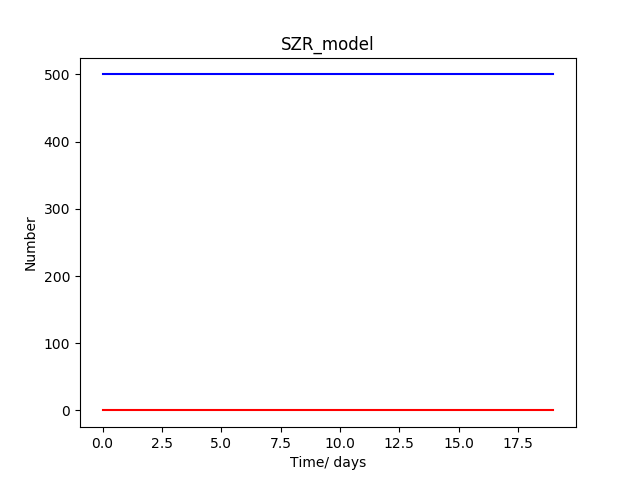
\includegraphics[width=10cm]{SZR/SZR_model1.png}
	\caption{The basic model in the case of no zombies, but this equilibrium is unstable.}
	\label{szr1graph}
\end{figure}
\begin{figure}[ht]
	\centering
	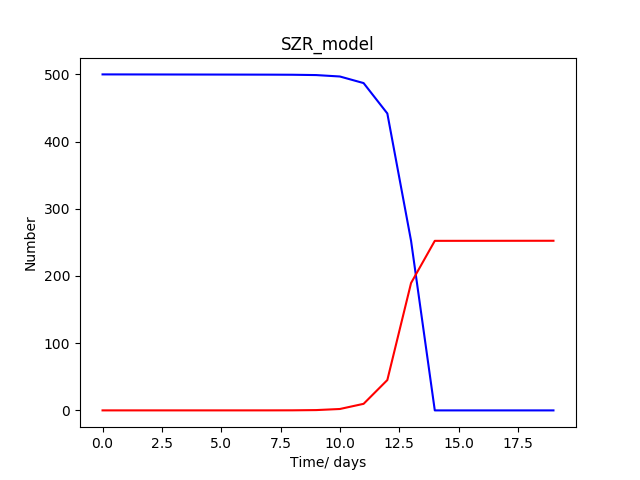
\includegraphics[width=10cm]{SZR/SZR_model2.png}
	\caption{The basic model. Suseptibles are quickly eradicated and zombies take over.}
	\label{szr2graph}
\end{figure}
Figures \ref{szr1graph} and \ref{szr2graph} shows the interaction between suseptibles and zombies over a period of time, we used Euler's method to solve the ODE's in pythin using the values $\alpha = 0.005$, $\beta = 0.0095$, $\zeta = 0.0001$, $\delta = 0.001$ in Figure \ref{szr2graph}.\newline

\subsection{SIZR model}
Next we revise this model to include a latent class of infeced individuals, a period of about 24 hours after the susecptible get sbitten befre they become a zombie. So we can extend the model \ref{szreqn} to include the possibility that a susecptible becomes infected before turnign to a zombie. So the changes to the basic model are:
\begin{itemize}
	\item Susceptibles first move to an infected class once infected and remain there for a period of time.
	\item Infected individuals can still die natural death before becoming a zombie.
\end{itemize}
This is called the SIZR model> the model is given by
\begin{eqnarray}
S^{'} &=& \prod - \beta SZ - \delta S \nonumber \\
I^{'} &=& \beta SZ- \rho I - \delta I\nonumber \\ 
Z^{'} &=& \rho I + \zeta R - \alpha SZ \nonumber \\
R^{'} &=& \delta S + \delta I + \alpha SZ - \zeta R.
\label{sizreqn}
\end{eqnarray}
 and is shown in Figure (\ref{sizr}).\newline
\begin{figure}[ht]
	\centering
	\includegraphics[width=15cm]{sizr.png}
	\caption{An SIZR model.}
	\label{sizr}
\end{figure}\newline
As before, if we set $\prod = \delta = 0$ and set equations \ref{sizreqn} equal to 0, we get
\begin{eqnarray}
0 &=& - \beta SZ \label{betaSZ}\\
0 &=& \beta SZ- \rho I \\ 
0 &=& \rho I + \zeta R - \alpha SZ \\
0 &=& \alpha SZ - \zeta R.
\label{sizreqn2}
\end{eqnarray}
Equation \ref{betaSZ} implies that $S=0$ or $Z=0$, meaning either all the humans are dead or all the zombies are dead, so there is no coexistnace possible which folows on from our basic model analysis. USing this we find the equiibria $(S, I, Z, R) = (0, 0, z, 0), (s, 0, 0, 0)$. Therefore our matrix is,
\begin{eqnarray}
J = 
\begin{pmatrix}
-\beta Z & 0 & -\beta S & 0 \\
\beta Z & -\rho & \beta S & 0 \\
-\alpha Z & \rho & -\alpha S & \zeta \\
\alpha Z & 0 & \alpha S & -\zeta \\
\end{pmatrix}
\end{eqnarray}
When we use $(S, I, Z, R) = (0, 0, z, 0)$ we get 
\begin{eqnarray}
J = 
\begin{pmatrix}
-\beta Z- \lambda & 0 & 0 & 0 \\
\beta Z & -\rho - \lambda & 0 & 0 \\
-\alpha Z & \rho & - \lambda & \zeta \\
\alpha Z & 0 & 0 & -\zeta - \lambda \\
\end{pmatrix}
\end{eqnarray} 
The eigenvalues are given by
\begin{eqnarray}
\det(J(0, 0, Z, 0)- \lambda I)&=&(-\beta Z - \lambda)\det\begin{pmatrix}
 -\rho - \lambda & 0 & 0 \\
 \rho & - \lambda & \zeta \\
 0 & 0 & -\zeta - \lambda \\
\end{pmatrix} \\
&=& (-\beta Z - \lambda)(-\rho - \lambda)\det\begin{pmatrix}
 - \lambda & \zeta \\
 0 & -\zeta - \lambda \\
\end{pmatrix} \\
&=&-\lambda (-\beta Z - \lambda)(-\rho - \lambda)(-\zeta - \lambda )
\end{eqnarray} 
Thefore the eigenvalues are $\lambda = 0$, $-\beta Z$, $-\rho$, $-\zeta$. As all the eigenvalues are non- positive then the doosmday equiibruim is stable.
When we use $(S, I, Z, R) = (S, 0, 0, 0)$ we get 
\begin{eqnarray}
J = 
\begin{pmatrix}
-\lambda &  0 & -\beta S & 0 \\
0 & -\rho - \lambda & \beta S & 0 \\
0 & \rho & -\alpha S - \lambda & \zeta \\
0 & 0 & \alpha S & -\zeta - \lambda \\
\end{pmatrix}
\end{eqnarray} 
The eigenvalues are given by
\begin{eqnarray}
\det(J(S, 0, 0, 0)- \lambda I)&=&-\lambda \det \begin{pmatrix}
-\rho - \lambda & \beta S & 0 \\
\rho & -\alpha S - \lambda & \zeta \\
0 & \alpha S & -\zeta - \lambda \\
\end{pmatrix}
-\beta S \det 
\begin{pmatrix}
0 & -\rho - \lambda & 0 \\
0 & \rho & \zeta \\
0 & 0 & -\zeta - \lambda \\
\end{pmatrix} \nonumber \\
&=& -\lambda((-\rho - \lambda)\det \begin{pmatrix}
-\alpha S - \lambda & \zeta \\
\alpha S & -\zeta - \lambda \\
\end{pmatrix} - \beta S \det \begin{pmatrix}
\rho & \zeta \\
0 & -\zeta - \lambda
\end{pmatrix}) \nonumber \\
&=& -\lambda((-\rho - \lambda)((-\alpha S - \lambda)(-\zeta - \lambda)-\alpha \zeta S)) - \beta \rho S(-\zeta- \lambda) \nonumber \\
&=& - \lambda((-\rho - \lambda)(\alpha S \zeta + \alpha S \lambda + \zeta \lambda + \lambda ^ 2 -\zeta \alpha S) +\beta S \rho \zeta  + \beta S \lambda \rho) \nonumber \\
&=& -\lambda(-\lambda^3 + \lambda^2(-\rho - \zeta -\alpha S) + \lambda(-\rho \alpha S - \rho \zeta + \beta S \rho) + \beta S \rho \zeta).
\end{eqnarray} 
As $\beta S \rho \zeta > 0$ then $\det(J(S, 0, 0, 0)- \lambda I)$ has an eigenvalue wit a positive real part, therefore teh disease-free equilibrium is unstable. 
\begin{figure}[ht]
	\centering
	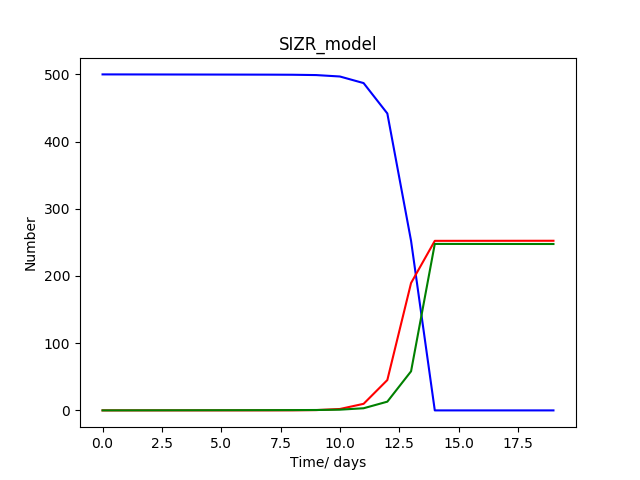
\includegraphics[width=15cm]{SZR/SIZR_model.png}
	\caption{An SIZR model.}
	\label{sizrgraph}
\end{figure}\newline
We then ploooted the numerical results using Euler's method to get Figure \ref{sizrgraph}. We found that even with the latent period of infection, zombies still take over but it takes twice as long as with no latent period.\newline

\subsection{SIZRQ model}
Next we look at what would happen if we tried to contain the outbreak. For example if we tried to keep the zombies in a qusarinted area away from the susepptibles so they cannot infect new individuals. Thefore the chages to the previuos model are:
\begin{itemize}
	\item The quarantined area only contains members of the infected or zombie populations.
	\item There is a chance some zombies wil try to escape the quaranitined area, but any that do so will be killed. 
	\item These killed individuals enter the removed class.
\end{itemize}
This is called the SIZRQ model, the model is given by,
\begin{eqnarray}
S^{'} &=& \prod - \beta SZ - \delta S \nonumber \\
I^{'} &=& \beta SZ- \rho I - \delta I\ -\kappa I \nonumber \\ 
Z^{'} &=& \rho I + \zeta R - \alpha SZ - \sigma Z \nonumber \\
R^{'} &=& \delta S + \delta I + \alpha SZ - \zeta R + \gamma Q \nonumber \\
Q^{'} &=& \kappa I + \sigma Z - \gamma Q.
\label{sizrqeqn}
\end{eqnarray}
\begin{figure}[ht]
	\centering
	\includegraphics[width=15cm]{sizrq.png}
	\caption{An SIZR model.}
	\label{sizrq}
\end{figure}\newline
and is shown in Figure \ref{sizrq}.
As before, if we set $\Pi = \delta = 0$ and set equations \ref{sizrqwqn} equal to 0, we get
\begin{eqnarray}
0 &=& - \beta SZ \label{betaSZ1}\\
0 &=& \beta SZ- \rho I -\kappa I \\ 
0 &=& \rho I + \zeta R - \alpha SZ -\sigma Z \\
0 &=& \alpha SZ - \zeta R + \gamma Q\\
0 &=& \kappa I + \sigma Z - \gamma Q.
\label{sizrqeqn2}
\end{eqnarray}
Equation \ref{betaSZ1} implies that $S=0$ or $Z=0$, meaning either all the humans are dead or all the zombies are dead, so there is no coexistnace possible which folows on from our basic model analysis. USing this we find the equiibria $(S, I, Z, R) = (0, 0, z, 0), (s, 0, 0, 0)$. Therefore our matrix is,



\section{To run or fight}
Next we will look at if there was a zombie emidemic if its better to run and hide or confront the ombies. Also whether suseptibles should contiue working, or learnt how to fight zombies? We will divide the human suseptibles into threepopulations: workers, who generate supplies; militia, who hunt and kill zombies; and moles, who seek to avoid confrontation by hiding. \newline
Suseptibles should be able to change their class according to circumsatnces. For example when a worker encounters a zombie and lives, there is a chance that the worker will join the militia, but there is also a chance that the worker will become a mole and hide from the zombies. Therefore our model is:

\begin{eqnarray}
S_z^{'} &=& z_1 \frac{S_wS_z}{N} + z_2 \frac{S_hS_z}{N} + (z_3 - M_1) \frac{S_mS_z}{N} \label{sz}\\
S_w^{'} &=& -(z_1 + \alpha(1-z_1) + \beta(1-z_1- \alpha(1-z_1)))\frac{S_zS_w}{N} + F_4S_w  - F_5\frac{S_wS_m}{N}\\
S_m^{'} &=& - z_3 \frac{S_z S_m}{N} + \beta(1-z_1-\alpha(1-z_1))\frac{S_zS_w}{N} - F_5 \frac{S_mS_m}{N} - \alpha(1-z_3) \frac{S_zS_m}{N} \nonumber \\&& + \beta(1-z_2)\frac{S_hS_z}{N} \\
S_h^{'} &=& - z_2 \frac{S_z S_h}{N} + \alpha(1-z_1)\frac{S_z S_w}{N} - F_5 \frac{S_h S_m}{N} + \alpha (1-z_3) \frac{S_z S_m}{N} \nonumber \\ &&- \beta (1-z_2) \frac{S_hS_z}{N} \label{sh}
\end{eqnarray}
Where $S_z$ denotes teh zombie popultaion, $S_w$ the worker population, $S_m$ the militia population and $S_h$ the hiding mole population and $N$ is the population density. $z_1$ is a value between 0 and 1 dicating how effective the avergae zombie will be at convertigng a worker, $z_2$ is a value between 0 and 1 dictating how effective a zombie is at converting a mole and $z_3$ is a value between 0 and 1 dictating how effective a zombie is at converting a militia. $M_1$ is teh avergae success that a militia will kill a zombie. $\alpha$ is the portion of the population that will zoin the mole community after seeing a zombie, $\beta$ is the portion of the population that will join the militia. $F_4$ is the overall birth-rate per day and $F_5$ is the odds that a person will accidently be shot by a militria member.\\
We can now perform stability analysis on these equations by settign equations \ref{sz} to \ref{sh} equal to 0. We can then construct the following matrix,
\begin{eqnarray}
\begin{pmatrix}
z_1 \frac{s_w}{N} + z_2 \frac{S_h}{N} + \theta\frac{S_m}{N} & z_1 \frac{S_z}{N} & \theta\frac{S_z}{N} & z_2 \frac{S_z}{N}\\
\gamma\frac{S_w}{N} & \gamma\frac{S_z}{N} + F_4 - F_5\frac{S_m}{N} & - F_5\frac{S_w}{N} & 0 \\
- (z_3 + \phi) \frac{S_m}{N} + \zeta\frac{S_w}{N} + \rho\frac{S_h}{N} & \zeta\frac{S_z}{N} & - (z_3+ \phi)\frac{S_z}{N} - F_5 \frac{S_m}{N} & \rho \frac{S_z}{N}\\
- (z_2 + \rho) \frac{ S_h}{N} + \omega\frac{S_w}{N} + \phi \frac{S_m}{N} &  \omega\frac{S_z}{N} & - F_5 \frac{S_h}{N} + \phi \frac{S_z}{N} & - F_5 \frac{S_m}{N} - (z_2 + \rho)\frac{S_z}{N}\\
\end{pmatrix}
\nonumber
\end{eqnarray}
Where $\gamma = -(z_1 + \alpha(1-z_1) + \beta(1-z_1- \alpha(1-z_1)))$, $\zeta = \beta(1-z_1-\alpha(1-z_1))$, $\phi = \alpha(1-z_3)$, $\rho = \beta (1-z_2)$, $\omega = \alpha(1-z_1)$ and $\theta = (z_3- M_1)$. We have an equiibrium at $(S_z, S_w, S_m, S_h) = (0, S_w, S_m, S_h)$. The Jacobian is:
\begin{eqnarray}
\begin{pmatrix}
z_1 \frac{s_w}{N} + z_2 \frac{S_h}{N} + \theta\frac{S_m}{N} - \lambda & 0 & 0 & 0\\
\gamma\frac{S_w}{N} & \gamma\frac{S_z}{N} + F_4 - F_5\frac{S_m}{N} - \lambda & - F_5\frac{S_w}{N} & 0 \\
- (z_3 + \phi) \frac{S_m}{N} + \zeta\frac{S_w}{N} + \rho\frac{S_h}{N} & 0 & - F_5 \frac{S_m}{N} - \lambda & 0\\
- (z_2 + \rho) \frac{ S_h}{N} + \omega\frac{S_w}{N} + \phi \frac{S_m}{N} &  0 & - F_5 \frac{S_h}{N} & - F_5 \frac{S_m}{N} - \lambda\\
\end{pmatrix}
\nonumber
\end{eqnarray}
Therefore the eigenvalues are $\lambda = z_1 \frac{s_w}{N} + z_2 \frac{S_h}{N} + \theta\frac{S_m}{N}$, $\lambda = \gamma\frac{S_z}{N} + F_4 - F_5\frac{S_m}{N}$, $\lambda = - F_5 \frac{S_m}{N}$ and $\lambda =  F_5 \frac{S_m}{N}$. As $F_5 \frac{S_m}{N} >0$ because the values $F_5$, $S_m$ and $N$ are all larger than 0, therefore the human existence in the absence of zombies is unstable.\\
We also have another equibrium at $(S_z, S_w, S_m, S_h) = (S_z, 0, 0, 0)$ this gives us 
\begin{eqnarray}
\begin{pmatrix}
- \lambda & z_1 \frac{S_z}{N} & \theta\frac{S_z}{N} & z_2 \frac{S_z}{N}\\
0 & \gamma\frac{S_z}{N} + F_4 - \lambda & 0 & 0 \\
0 & \zeta\frac{S_z}{N} & - (z_3+ \phi)\frac{S_z}{N} - \lambda & \rho \frac{S_z}{N}\\
0 &  \omega\frac{S_z}{N} & \phi \frac{S_z}{N} & - (z_2 + \rho)\frac{S_z}{N} - \lambda\\
\end{pmatrix}
\nonumber
\end{eqnarray}
The determinant and the eigenvalues can be calculated by 
\begin{eqnarray}
-\lambda \det
\begin{pmatrix}
\gamma\frac{S_z}{N} + F_4 - \lambda & 0 & 0 \\
\zeta\frac{S_z}{N} & - (z_3+ \phi)\frac{S_z}{N} - \lambda & \rho \frac{S_z}{N}\\
\omega\frac{S_z}{N} & \phi \frac{S_z}{N} & - (z_2 + \rho)\frac{S_z}{N} - \lambda\\
\end{pmatrix}
\nonumber \\- z_1 \frac{S_z}{N} \det
\begin{pmatrix}
0  & 0 & 0 \\
0  & - (z_3+ \phi)\frac{S_z}{N} - \lambda & \rho \frac{S_z}{N}\\
0  & \phi \frac{S_z}{N} & - (z_2 + \rho)\frac{S_z}{N} - \lambda\\
\end{pmatrix}
+ \theta \frac{S_z}{N} \det
\begin{pmatrix}
0 & \gamma\frac{S_z}{N} + F_4 - \lambda & 0 \\
0 & \zeta\frac{S_z}{N} & \rho \frac{S_z}{N}\\
0 &  \omega\frac{S_z}{N} & - (z_2 + \rho)\frac{S_z}{N} - \lambda\\
\end{pmatrix}
\nonumber \\ -z_2 \frac{S_z}{N} \det
\begin{pmatrix}
0 & \gamma\frac{S_z}{N} + F_4 - \lambda & 0  \\
0 & \zeta\frac{S_z}{N} & - (z_3+ \phi)\frac{S_z}{N} - \lambda\\
0 &  \omega\frac{S_z}{N} & \phi \frac{S_z}{N}\\
\end{pmatrix} \nonumber \\
= -\lambda (\gamma\frac{S_z}{N} + F_4 - \lambda) \det
\begin{pmatrix}
 - (z_3+ \phi)\frac{S_z}{N} -\lambda & \rho \frac{S_z}{N}\\
 \phi \frac{S_z}{N} & - (z_2 + \rho)\frac{S_z}{N} - \lambda\\
\end{pmatrix}
\end{eqnarray}
this shows 
\begin{eqnarray}
 &=& -\lambda (\gamma\frac{S_z}{N} + F_4 - \lambda)((- (z_3+ \phi)\frac{S_z}{N} -\lambda)(- (z_2 + \rho)\frac{S_z}{N} - \lambda)- (\rho \frac{S_z}{N})(\phi \frac{S_z}{N})) \nonumber \\
 &=& -\lambda (\gamma\frac{S_z}{N} + F_4 - \lambda)(\frac{S_z^2}{N^2}(z_2z_3 + \rho z_3 + \phi z_2) + \lambda \frac{S_z}{N}(z_3 + \phi + z_2 + \rho) + \lambda ^ 2) \nonumber \\
 &=& -\lambda \gamma \frac{S_z ^ 3}{N^3}(z_2z_3 + \rho z_3 + \phi z_2) -\lambda ^2 \gamma \frac{S_z ^ 2}{N^2}(z_3 + \phi + z_2 + \rho) -\lambda ^3 \gamma \frac{S_z}{N} -\lambda F_4(\frac{S_z^2}{N^2}(z_2z_3 + \rho z_3 + \phi z_2)\nonumber\\&& - \lambda F_4(z_3 + \phi + z_2 + \rho) - \lambda^3 F_4  + \lambda ^2(\frac{S_z^2}{N^2}(z_2z_3 + \rho z_3 + \phi z_2) + \lambda^2 \frac{S_z}{N}(z_3 + \phi + z_2 + \rho) + \lambda ^ 4 \nonumber \\
 &=& \lambda ^ 4 + \lambda ^ 3(-\gamma \frac{S_z}{N} - F_4) + \lambda ^2(\gamma \frac{S_z ^ 2}{N^2}(z_3 + \phi + z_2 + \rho)+ \frac{S_z^2}{N^2}(z_2z_3 + \rho z_3 + \phi z_2)+ \frac{S_z}{N}(z_3 + \phi + z_2 + \rho))  \nonumber \\ &&  + \lambda(\gamma \frac{S_z ^ 3}{N^3}(z_2z_3 + \rho z_3 + \phi z_2)- F_4\frac{S_z^2}{N^2}(z_2z_3 + \rho z_3 + \phi z_2)- F_4(z_3 + \phi + z_2 + \rho) )
\end{eqnarray}
\begin{thebibliography}{99}
	\bibitem{Prior}
	Christopher Prior. {\it  Math Biology lecture notes and questions.} \url{https://duo.dur.ac.uk/ }
	\bibitem{Munz}
	Philip Munz, Ioan Hudea, Joe Imad, Robert J. Smith. {\it  When zombies attack!:  Mathematical modelling of an outbreak of zombie infection.} \url{https://www.loe.org/images/content/091023/Zombie%20Publication.pdf}
	\bibitem{Strickland}
	Christopher Strickland. {\it Modelling the Dynamics of a zombie breakout.} \url{https://www.samsi.info/wp-content/uploads/2016/02/Zombies.pdf}
\end{thebibliography}
\end{document}
